\documentclass{article}
\usepackage{graphicx} % Required for inserting images
\usepackage{amsmath}
\usepackage{amsfonts}
\usepackage{multicol}
\usepackage{float}
\usepackage[a4paper, left=26mm,top=26mm,right=26mm,bottom=26mm]{geometry}

\title{CTA200 Assignment 3 Report}
\author{Jewel Cao}

\begin{document}

\maketitle
\begin{multicols}{2}

\section{Question 1}

To designate a criteria for "divergence", I imposed the restriction that successive iterations must not exceed a given tolerance, which I set as 1e6. I created a function named 'complex\_iterate' which would return the iteration number i where the $z_{i+1} - z_i > 1e6$, and 'None' if the tolerance was never exceeded. I created a contour graph indicating the number of iterations needed to exceed the tolerance (Figure 1). 

Since I had produced an array with the iteration number of divergence for values in $\{c \in \mathbb{C} : -2 < Re(c), Im(c) < 2\}$, I replaced all the values of the array that were greater than 0 with a fixed constant of 10. Then, all the values of 10 corresponded to points that "diverged". I plotted this on another contour graph (Figure 2). 

\begin{figure} [H]
    \centering
    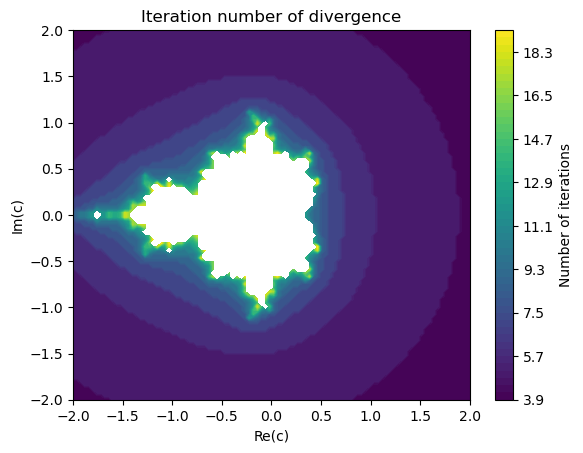
\includegraphics[width=1.0\linewidth]{Assignment 3 Images/download.png}
    \caption{Contour graph indicating the number of iterations of $z_{n+1} = z_{n}^2 + c$ required for the difference between successive iterations to exceed the given tolerance of 1e6, for values of c in the set $\{c \in \mathbb{C} : -2 < Re(c), Im(c) < 2\}$. White indicates that the tolerance was not exceeded, and the given point converges.}
    \label{fig:enter-label}
\end{figure}

\begin{figure} [H]
    \centering
    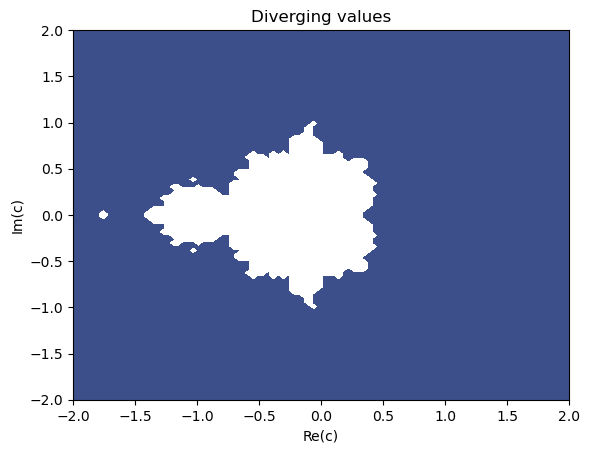
\includegraphics[width=1.0\linewidth]{Assignment 3 Images/download (1).png}
    \caption{Contour graph indicating whether the iterative sequence $z_{n+1} = z_{n}^2 + c$ converges for given value of c, with c in the set $\{c \in \mathbb{C} : -2 < Re(c), Im(c) < 2\}$. White indicates that the given point converges, while blue indicates that the point diverges.}
    \label{fig:enter-label}
\end{figure}

\section{Question 2}

I created a function that returned the right hand side of the Lorenz ODEs, and used solve\_ivp for this question. I reproduced Lorenz' Figures 1 and 2 (Figures 3, 4, and 5) by closely following the process described in the assignment instructions. 

In Figure 3, I plotted the timeseries of the Y component of the solution W over the entire time interval where I applied solve\_ivp. In Figures 4 and 5, I used numpy linspace to 'smooth out' the solutions by applying more iterations (1000) in a smaller time interval. 

In order to produce Figure 6, I repeated my previous steps to solve the ODE with slightly different initial conditions $W_0'$. I subtracted the two solutions W and W' to create a new array W\_diff to represent the vector difference between the two solutions. Then I used the numpy linalg norm function on W\_diff to calculate the scalar distance between the two solutions, which I plotted with the semilogy function in matplotlib. 

As expected, Figures 3, 4, and 5 look similar to Lorenz' figures. However, Lorenz' figures were probably created over a slightly different time interval, since I was unable to specify the exact iteration numbers desired on solve\_ivp. As a consequence, my figures are also plotted over units of time rather than iterations. Figure 6 appears linear on the semilog plot between units of time 0 to 40, at which point it plateaus. This suggests exponential growth of the small difference in initial condition between W and W' over this period, before diminishing into a linear increase in difference. 

\begin{figure} [H]
    \centering
    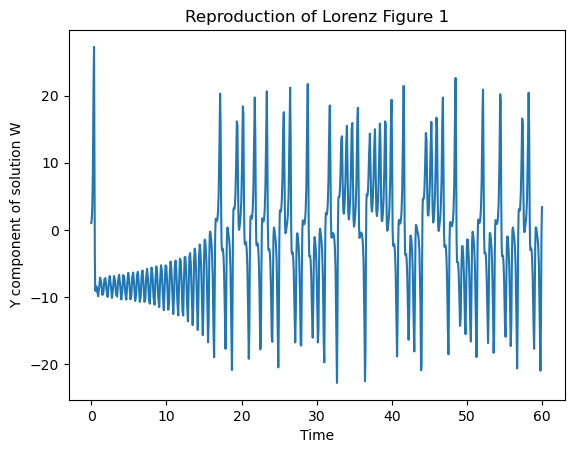
\includegraphics[width=1.0\linewidth]{Assignment 3 Images/download (2).png}
    \caption{Y component of solution to Lorenz equations W over time, with initial parameters $\sigma$, $r$, $b$ and initial conditions $W_0$ as described in assignment instructions.}
    \label{fig:enter-label}
\end{figure}

\begin{figure} [H]
    \centering
    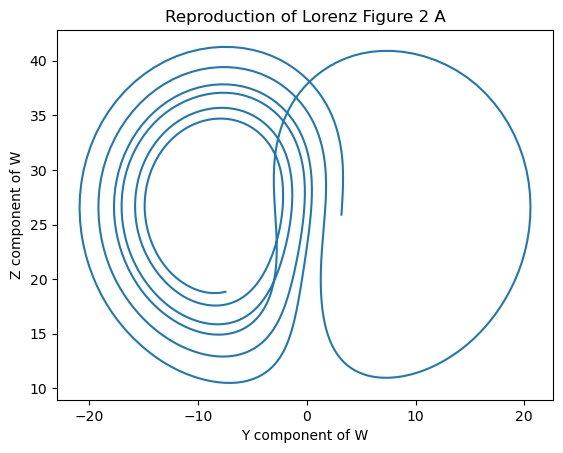
\includegraphics[width=1.0\linewidth]{Assignment 3 Images/download (3).png}
    \caption{Phase space diagram of Y and Z components of solution to Lorenz equations W, between 14 and 19 units of time, with 1000 iterations, with initial parameters and initial conditions of Figure 2.}
    \label{fig:enter-label}
\end{figure}

\begin{figure} [H]
    \centering
    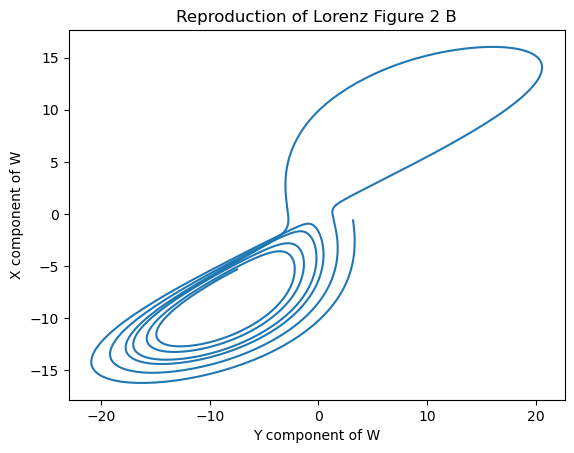
\includegraphics[width=1.0\linewidth]{Assignment 3 Images/download (4).png}
    \caption{Phase space diagram of Y and X components of solution to Lorenz equations W, between 14 and 19 units of time, with 1000 iterations, with initial parameters and initial conditions of Figure 2.}
    \label{fig:enter-label}
\end{figure}

\begin{figure} [H]
    \centering
    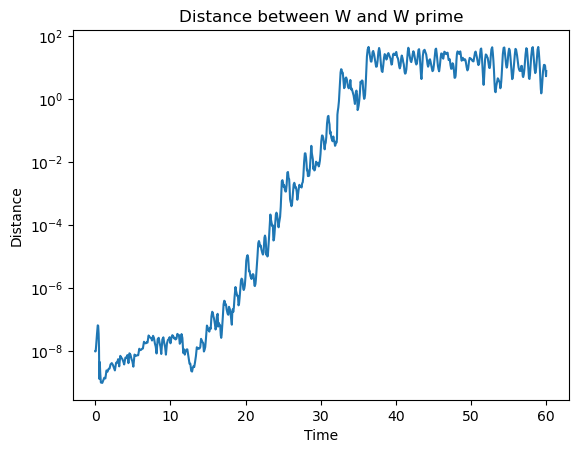
\includegraphics[width=1.0\linewidth]{Assignment 3 Images/download (5).png}
    \caption{Norm of difference between solution W generated with initial conditions as in Figures 4 and 5 and solution W' generated with initial conditions $X = 0$, $Y = 1.e-8$, $Z=0$.}
    \label{fig:enter-label}
\end{figure}

\end{multicols}
\end{document}
